
\newcommand{\hc}{h_\text{c}}
\newcommand{\hf}{h_\text{f}}

\newcommand{\sigmafail}{\sigma_\text{y}}
\newcommand{\taufail}{\tau_\text{y}}
\newcommand{\tauz}{\tau_\text{yZ}}

\begin{figure}[H]
	\centering
	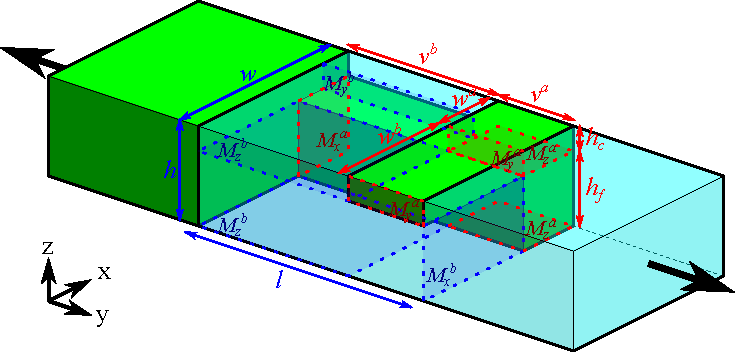
\includegraphics[width=\columnwidth]{sources/method/straight_model_v3.pdf}
	\caption{
		One straight unit cell connecting material $a$ (left) to material $b$ (right).
		Failure can happen along the fingers ($M_x$), along the cross beams ($M_y$) or at the interface between the two ($M_z$) for either material.}
	\label{fig:failure_modes}
\end{figure}


\section{Straight design}

\iffalse
The bending constraint is given by:
\begin{align*}
	\sigma_\text{max} &= \frac{M}{I}c \\
	c &= \nicefrac12 h \\
	I &= \frac{b h^3}{12} \\
	M &= \frac{w L^2}{12} \\
	w &= \frac{F}{L} \\
	\sigma_\text{max} &= \frac{w L^2 / 12}{b h^3 / 12} \nicefrac12 h \\
	\sigma_\text{max} &= \frac{w L^2}{b h^3} \nicefrac12 h \\
	\sigma_\text{max} &= \frac{F L}{b h^3} \nicefrac12 h \\
	\sigma_\text{max} &= \frac{F L}{2 b h^2} \\
\end{align*}
\fi


\Cref{fig:failure_modes} shows one cell of the straight structure, along with the design variables and the failure modes.
We want to optimize the effective ultimate tensile strength, while keeping the structure minimal.
The optimization problem can be formulated as follows:

\begin{align}
	& \omit\rlap{$\displaystyle \max{ \frac{F}{\left( w^a + w^b \right) \left( \hf + \hc \right) }}$} \label{eq:obj} \\
	& \omit\rlap{$\displaystyle \min{ \hf + \hc} $} \nonumber \\
	& \omit\rlap{$\displaystyle \min{ w^a + w^b} $} \nonumber \\
	\omit\rlap{subject to} \nonumber \\
	w^m &\ge 2 \wmin^m			&&\text{ Nozzle size} \label{eq:c1} \\
	v^m &\ge \wmin^m				&&\text{ Nozzle size}  \label{eq:c2} \\
	\hf &\ge \hmin		&&\text{ Layer thickness}  \label{eq:c3} \\
	\hc &\ge \hmin		&&\text{ Layer thickness}  \label{eq:c4} \\
	v^a + v^b &\le \lmax         &&\text{ Design constraint}   \label{eq:c_total_length} \\
	\sigma_{11}^m = \frac{ F }{ w^m \hf } &\le \sigmafail^m					&&\text{ Tension failure } M_x^m  \label{eq:c_tensile} \\
	\sigma_{13}^m = \frac{ F w^{\neg m} }{ 2 v^m \hc w } &\le \taufail^m					&&\text{ Shear failure } M_y^m  \label{eq:c_shear} \\
	\sigma_{22}^m = \frac{ F \left(w^{\neg m}\right)^2 }{ 2 \left( v^m \right)^2 \hc w } &\le \sigmafail^a                 &&\text{ Bending failure } M_y^m  \label{eq:c_bending} \\
	\sigma_{12}^m = \frac{ F }{ 2 v^m w^m} &\le \tauz^m							&&\text{ Shear failure } M_z^m  \label{eq:c_shear_z} \\
	\omit\rlap{for both materials $m \in \{a, b\}$ where $\neg a = b$ and $\neg b = a$}\nonumber
\end{align}

The first objective function is the main objective; 
the other two objective functions are secondary.
They are only introduced to disambiguate designs which have the same value for the objective function --
that is: pareto optimality is introduced to disambiguate otherwise equivalent designs.

Note that the $v^m$ variables don't figure in the objective,
but they do appear in the constraints and therefore are also subject to the optimization.
Some of the mechanical constraints will be active to provide them a definite value.

\subsection{Stress formulae}
Let's consider the stresses $\sigma$ induced by applying a force to the ends of the unit cell.
Tensile stress in the finger of either material $m$ is given by:
\begin{align*}
	\sigma_{11}^m &= \frac{ F }{ w^m \hf }
\end{align*}

The shear stress acting on $M_y^m$ for either material $m$ is determined by modeling the unsupported portion of the cross beam as a doubly fixed beam,
whereas the total load is modeled as being uniformly distributed over the whole beam.
The portion of the total force $F$ which acts upon the unsupported part of material $a$ is proportional to $w^b / w$.
Because the beam is fixed on both sides the shear force is half the total force acting on the beam.
\begin{align*}
	\sigma_{13}^m = \frac{F w^{\neg m} / w}{2 v^m \hc} = \frac{F w^{\neg m}}{2 v^m \hc w}
\end{align*}
where $w = w^a+w^b$.

The same unsupported portion of the cross beam might be subject to bending.
The highest bending stress for a doubly supported beam will occur on either end.
\begin{align*}
	\sigma_{22}^m &= \frac{M}{I}c = \frac{(F w^{\neg m} / w) w^{\neg m} / 12}{\hc (v^m)^3 / 12} \nicefrac12 v^m =  \frac{ F \left(w^{\neg m}\right)^2 }{ 2 \left( v^m \right)^2 \hc w }
\end{align*}

There is also a shear stress acting along the surface $M_z^m$.
While one might think that only a portion of the total force $F$ is working on the supported portion of the cross beam,
the total force must be enacted through this plane, because it is the only connection between the finger and the cross beam.
The shear stress along the Z direction is therefore given by:
\begin{align*}
	\sigma_{12}^m = \frac{ F }{ 2 v^m w^m}
\end{align*}


\subsection{Constraint values}
Under different circumstances the values of the constraints will be different.
Different nozzles and different layer thickness settings require different constraint values.
Because of manufacturing constraints we know that the layer thickness has to be smaller than half the smallest nozzle size:
$\hmin < \nicefrac{1}{2} \wmin^m$.

Materials properties of 3D printed materials are always such that $\tauz^m < \taufail^m$.
According to the von Mises yield criterion we have that $\taufail^m = \sigmafail^m / \sqrt{3} $.

Depending on the types of material used the tensile and shear strength in the Z direction can be an order of magnitude lower than in the horizontal directions.
In such a case the Z shearing failure constraints \cref{eq:c_shear_z} will be active for that material.

Depending on the design we might apply a different $\lmax$, 
but it is required that $\lmax \ge \wmin^a + \wmin^b$.

\subsection{Boundedness}
The manufacturing constraints provide sufficient lower bounds, but the upper bounds are problematic in the current formulation.
The design constraint effectively places an upper bound on the $v^m$ widths.
One might think that this constraint drives the other design variables to some finite value as well.
However, in this section we show how the current formulation will be amended to make the problem well-behaved.

\label{sec:domain_assumptions}
If we would scale all design variables linearly with some factor $R$ and $F$ by $R^2$ then the objective function and all mechanical constraints \crefrange{eq:c_tensile}{eq:c_shear_z} remain at the same value.
If only those constraints were to be considered the problem would have been under-constrained.
Since one of our objective functions is to minimize the total width $(w^a + w^B)$ we know that some of the constraints \crefrange{eq:c1}{eq:c4} will have to be active.
If we set \cref{eq:c1} active for material $a$ we will show that none of the other constraints will be violated, so this constraint has to be active.

The same holds for the heights.
We can scale $\hc$, $\hf$ and $F$ down with a factor $R$ without changing the value of the objective function nor the mechanical constraints \crefrange{eq:c_tensile}{eq:c_bending}.
The Z shear constraint \cref{eq:c_shear_z} does change, but as long as we scale down $R<1$ this constraint will remain satisfied.
This means the problem definition is not well-defined.
In order to solve this we use the height objective function $(\hf + \hc)$ to set \cref{eq:c4} active and we will show that \cref{eq:c3} is not violated.


\paragraph{Constraint redundancy}
If $\nicefrac{w^b}{v^a} > \nicefrac{ \sigmafail^a }{ \taufail^a } = \sqrt{3}$ 
then the shear failure constraints \cref{eq:c_shear} for material $a$ is dominated by the bending failure constraint \cref{eq:c_bending},
since then 
$
\frac{ F w^b }{ 2 \left( v^a \right)^2 \hc \sigmafail^a}
> \frac{ F }{ 2 v^a \hc \taufail^a} 
$.
Otherwise the latter is dominated by the former.
The same holds conversely with the materials $a$ and $b$ swapped.
Therefore two of \cref{eq:c_shear,eq:c_bending,eq:c_bending} will be redundant.
We could combine those four constraints into two single ones:
\begin{align}
	%\frac{ F }{ 2 v^m \hc} &\le \taufail^m \\
	%\frac{ F }{ 2 v^m \hc} &\le \nicefrac1{\sqrt{3}} \sigmafail^m \\
	%\frac{ F }{ 2 \cdot \sqrt{3} v^m \hc} &\le \sigmafail^m \\
	%???\frac{ F w^b }{ 2 \left( v^a \right)^2 \hc } &\le \sigmafail^a \\
	%\\
	\frac{ F }{ 2 v^a \hc }  \max{\left( \sqrt{3}, \frac{w^b}{ v^a} \right)} &\le \sigmafail^a  \nonumber \\
	\frac{ F }{ 2 v^b \hc }  \max{\left( \sqrt{3}, \frac{w^a}{ v^b} \right)} &\le \sigmafail^b  \label{eq:shear_bend_combined}
\end{align}


\paragraph{Von Mises criterion}
However, when these criteria are near-active then there could be an interaction between the two.
The shear and bending interact and thereby lower the force at which failure happens.
In order to estimate the combined failure criterion we consider the von Mises yield criterion.
When only considering one tensile stress and one shear stress, the criterion reduces to:

\begin{align*}
	% \sqrt{\frac12 \left(  \left(\sigma_{11} - \sigma_{22}\right)^2  +  \left(\sigma_{22} - \sigma_{33}\right)^2  +  \left(\sigma_{33} - \sigma_{11}\right)^2   +   6\left(\sigma_{23}^2 + \sigma_{13}^2 + \sigma_{12}^2\right)\right)}&< \sigmafail \\
	%\sqrt{\frac12 \left(  \left(\sigma_{11} \right)^2  +  \left( - \sigma_{11}\right)^2   +   6\left(\sigma_{23}^2 \right)\right)}&< \sigmafail \\
	%\sqrt{\frac12 \left(  2 \left(\sigma_{11} \right)^2  +   6\left(\sigma_{23} \right)^2  \right)}&< \sigmafail \\
	%\sqrt{\frac12 \left(  2 \sigma ^2  +   6 \tau^2  \right)}&< \sigmafail \\
	\sqrt{ \sigma ^2  +   3 \tau^2 }&< \sigmafail
\end{align*}

Applied to our shear and bending, we get:

\begin{align}
	% \sqrt{ \left(  \frac{ F w^b }{ 2 \left( v^a \right)^2 \hc }  \right)^2   +   3 \left(  \frac{ F }{ 2 v^a \hc}  \right)^2 } &< \sigmafail^a \\
	% \sqrt{ \left(  \frac{ F }{ 2 v^a \hc} \frac{w^b}{v^a}  \right)^2   +   3 \left(  \frac{ F }{ 2 v^a \hc}  \right)^2 } &< \sigmafail^a \\
	% \sqrt{ \left(  \frac{ F }{ 2 v^a \hc}\right)^2  \left( \frac{w^b}{v^a}  \right)^2   +   3 \left(  \frac{ F }{ 2 v^a \hc}  \right)^2 } &< \sigmafail^a \\
	% \sqrt{ \left(  \frac{ F }{ 2 v^a \hc}\right)^2  \left( \left( \frac{w^b}{v^a}  \right)^2   +   3  \right) } &< \sigmafail^a \\
	\frac{ F }{ 2 v^a \hc} \sqrt{   \left( \frac{w^b}{v^a}  \right)^2 + 3 } &< \sigmafail^a \nonumber \\
	\frac{ F }{ 2 v^b \hc} \sqrt{   \left( \frac{w^a}{v^b}  \right)^2 + 3 } &< \sigmafail^b \label{eq:shear_bend_von_mises}
\end{align}

Note that the von Mises yield criterion \cref{eq:shear_bend_von_mises} is de facto equivalent to the application of the P-norm smooth approximation of the maximum function as used in the combined constraint \cref{eq:shear_bend_combined}, for $P=2$.
What a neat coincidence!
Where $\nicefrac{w^b}{v^a} \to 0$ and $\nicefrac{w^b}{v^a} \to \infty$ the failure is dominated by shear and bending respectively. 
This shows that in the limits the von Mises yield criterion and the combined criterion coincide.


Now let's consider the intersection where failure modes $M_x$, $M_y$ and $M_z$ meet.
At that particular corner all three failure modes act at once, so let's set up the von Mises yield criterion for that.

\begin{align*}
	\sigma_{12} &= \frac{ F }{ 2 v^m w} \\
	\sigma_{13} &= \frac{ F w^{\neg m} }{ 2 v^m \hc w }  =  \sigma_{12} \frac{w^{\neg m}}{\hc} \\
	\sigma_{11} &= \frac{ F }{ w^m \hf } \\
	\sigma_{22} &= \frac{ F \left(w^{\neg m}\right)^2 }{ 2 \left( v^m \right)^2 \hc w }   =   \sigma_{12} \frac{\left(w^{\neg m}\right)^2}{v^m \hc} = \sigma_{13} \frac{w^{\neg m}}{v^m}
\end{align*}

\begin{align*}
	%	\sqrt{\frac12 \left(  \left(\sigma_{11} - \sigma_{22}\right)^2  +  \left(\sigma_{22} - \sigma_{33}\right)^2  +  \left(\sigma_{33} - \sigma_{11}\right)^2   +   6\left(\sigma_{23}^2 + \sigma_{13}^2 + \sigma_{12}^2\right)\right)}&< \sigmafail \\
	%	\sqrt{\frac12 \left(  \left(\sigma_{11} - \sigma_{22}\right)^2  +  \sigma_{22}^2  +  \sigma_{11}^2   +   6\left(\sigma_{13}^2 + \sigma_{12}^2\right)\right)}&< \sigmafail \\
	%	\sqrt{\frac12 \left(  \sigma_{11}^2 + \sigma_{22}^2 - 2\sigma_{11}\sigma_{22} +  \sigma_{22}^2  +  \sigma_{11}^2   +   6\left(\sigma_{13}^2 + \sigma_{12}^2\right)\right)}&< \sigmafail \\
	\sqrt{  \sigma_{11}^2  +  \sigma_{22}^2  - \sigma_{11}\sigma_{22} +   3\left(\sigma_{13}^2 + \sigma_{12}^2\right)}&< \sigmafail \\
	%\sqrt{  \sigma_{11}^2  +  \sigma_{22}^2  - \sigma_{11}\sigma_{22} +   3\left( \left( \sigma_{12} \frac{w^{\neg m}}{\hc} \right)^2 + \sigma_{12}^2\right)}&< \sigmafail \\
	%\sqrt{  \sigma_{11}^2  +  \sigma_{22}^2  - \sigma_{11}\sigma_{22} +   3\sigma_{12}^2 \left( \left( \frac{w^{\neg m}}{\hc} \right)^2 + 1\right)}&< \sigmafail \\
	%\sigma_{11}^2  +  \sigma_{22}^2  - \sigma_{11}\sigma_{22} +   3\sigma_{12}^2 \left( \left( \frac{w^{\neg m}}{\hc} \right)^2 + 1\right) &< \sigmafail^2 \\
	%\sigma_{11}^2  +  \left(\sigma_{12} \frac{\left(w^{\neg m}\right)^2}{v^m \hc}\right)^2  - \sigma_{11}\sigma_{22} +   3\sigma_{12}^2 \left( \left( \frac{w^{\neg m}}{\hc} \right)^2 + 1\right) &< \sigmafail^2 \\
	%\sigma_{11}^2  +  \sigma_{12}^2 \left(\frac{\left(w^{\neg m}\right)^2}{v^m \hc}\right)^2  - \sigma_{11}\sigma_{22} +   3\sigma_{12}^2 \left( \left( \frac{w^{\neg m}}{\hc} \right)^2 + 1\right) &< \sigmafail^2 \\
	%\sigma_{11}^2  +  \sigma_{12}^2 \left(\frac{\left(w^{\neg m}\right)^2}{v^m \hc}\right)^2  - \sigma_{11}\sigma_{22} +   \sigma_{12}^2 \left( 3\left( \frac{w^{\neg m}}{\hc} \right)^2 + 3\right) &< \sigmafail^2 \\
	%\sigma_{11}^2  - \sigma_{11}\sigma_{22} +   \sigma_{12}^2 \left(  \left(\frac{\left(w^{\neg m}\right)^2}{v^m \hc}\right)^2  +   3\left( \frac{w^{\neg m}}{\hc} \right)^2 + 3\right) &< \sigmafail^2 \\
	%\sigma_{11}^2  - \sigma_{11}\sigma_{22} +   \sigma_{12}^2 \left(  \left(\frac{w^{\neg m}}{v^m}\right)^2  \left(\frac{w^{\neg m}}{\hc}\right)^2  +   3\left( \frac{w^{\neg m}}{\hc} \right)^2 + 3\right) &< \sigmafail^2 \\
	\sigma_{11}^2  - \sigma_{11}\sigma_{22} +   \sigma_{12}^2 \left(  \left(\frac{w^{\neg m}}{\hc}\right)^2  \left(  \left(\frac{w^{\neg m}}{v^m}\right)^2  +  3 \right) + 3\right) &< \sigmafail^2 \\
	\sigma_{11}^2  - \sigma_{11}\sigma_{22} +   \sigma_{12}^2 U &< \sigmafail^2 \\
	\left(\frac{ F }{ w^m \hf }\right)^2  - \frac{ F }{ w^m \hf } \frac{ F \left(w^{\neg m}\right)^2 }{ 2 \left( v^m \right)^2 \hc w }   +   \left(\frac{ F }{ 2 v^m w}\right)^2 U &< \sigmafail^2 \\
	\left(\frac{ 1 }{ w^m \hf }\right)^2  - \frac{ 1 }{ w^m \hf } \frac{ \left(w^{\neg m}\right)^2 }{ 2 \left( v^m \right)^2 \hc w }   +   \left(\frac{ 1 }{ 2 v^m w}\right)^2 U &< \frac{\sigmafail^2}{F^2} \\
	\left(\frac{ 1 }{ w^m \hf }\right)^2  - \frac{ \left(w^{\neg m}\right)^2 }{ 2 \left( v^m \right)^2 \hc w w^m \hf}   +   \left(\frac{ 1 }{ 2 v^m w}\right)^2 U &< \frac{\sigmafail^2}{F^2} \\
\end{align*}




\paragraph{Constraint validity}
A careful analysis of the geometry will show that once shearing failure mode $M_x^a$ has occurred, 
there is still interlocking between the two materials;
once part of the cross beams has sheared off, still a column of material $a$ remains, which is surrounded by material $b$.
Once one of those failure modes has occurred still any other failure mode has to occur for the interlock to fail, except $M_x^b$.
The only constraint added by the shearing failure modes should therefore be that both those failure modes occur together.
The constraint is violated only when both occur, so it is satisfied when either failure mode is prevented.
The logical disjunction can be rewritten into a minimum when both constraints are transformed into negative null form:
\begin{align*}
	% \min \left(  \frac{ F }{ 2 v^a \hc \sigmafail^a} \sqrt{   \left( \frac{w^b}{v^a}  \right)^2 + 3 }  ,  \frac{ F }{ 2 v^b \hc \sigmafail^b} \sqrt{   \left( \frac{w^a}{v^b}  \right)^2 + 3 }  \right) - 1 &< 0 \\
	% \frac{ F }{ 2 \hc}  \min \left(  \frac{ 1 }{ v^a \sigmafail^a} \sqrt{   \left( \frac{w^b}{v^a}  \right)^2 + 3 }  ,  \frac{ 1 }{ v^b \sigmafail^b} \sqrt{   \left( \frac{w^a}{v^b}  \right)^2 + 3 }  \right) - 1 &< 0 \\
	\frac{ F }{ 2 \hc}  \min \left(  \frac{ \sqrt{   \left( \frac{w^b}{v^a}  \right)^2 + 3 } }{ v^a \sigmafail^a}   ,  \frac{  \sqrt{   \left( \frac{w^a}{v^b}  \right)^2 + 3 } }{ v^b \sigmafail^b}  \right) - 1 &< 0 \\
	% \frac{ F }{ 2 \hc}  \min \left(  \frac{ \sqrt{   \left(w^b\right)^2 + 3 \left(v^a\right)^2 } }{ \left(v^a\right)^2 \sigmafail^a}   ,  \frac{  \sqrt{   \left(w^a\right)^2 + 3 \left(v^b\right)^2 } }{ \left(v^b\right)^2 \sigmafail^b}  \right) - 1 &< 0 \\
\end{align*}

Depending on the optimization algorithm used, the min operator might need to be replaced by smooth versions.
The choice between P-norm, Kreisselmeier-Steinhauser function or any of the other alternatives might be decided by properties of their derivatives.
The height of the $P$ value will determine the approximation error.
The approximation error of the max function means that the approximated constraint is more strict than the underlying sub-constraints, 
while the smooth approximation of the min function is more lenient.
This means that using a smooth approximation of this constraint could result in infeasible designs according to the analytical constraint.


\todo{TODO: rescale objective function so that they are approximately in the range 0-1.}

\todo{TODO: should we invert the mechanical constriants, so that the F is below the division line?}

\subsection{Problem reformulation}
Taking the above into account we reformulate the problem.
The shear constraints are combined into one.
The constraints which hold for both materials are expanded.
The variables set by the presumed to be active constraints are substituted.

We divide by the constraint values and invert the division of the mechanical constraints.
That way the formulae of those constraints are more alike and simpler to differentiate.

\newcommand{\gwb}{g_\text{wb}}
\newcommand{\gva}{g_\text{va}}
\newcommand{\gvb}{g_\text{vb}}
\newcommand{\ghf}{g_\text{hf}}
\newcommand{\gd}{g_\text{d}}
\newcommand{\gta}{g_\text{ta}}
\newcommand{\gtb}{g_\text{tb}}
\newcommand{\gc}{g_\text{c}}
\newcommand{\gza}{g_\text{za}}
\newcommand{\gzb}{g_\text{zb}}

\begin{align*}
	f: & \min{ \frac{\left( 2 \wmin^a + w^b \right) \left( \hf + \hmin \right) }{F} }\\
	\gwb: & 1 - \nicefrac{w^b }{2 \wmin^b} \le 0 \\
	\gva: & 1 - \nicefrac{v^a }{\wmin^a} \le 0 \\
	\gvb: & 1 - \nicefrac{v^b }{\wmin^b} \le 0 \\
	\ghf: & 1 - \nicefrac{\hf}{\hmin} \le 0 \\
	\gd: & \frac{v^a + v^b}{ \lmax }  - 1 \le 0 \\
	\gta: & 1 - \frac{ 2 \wmin^a \hf \sigmafail^a }{ F } \le 0 \\
	\gtb: & 1 - \frac{ w^b \hf \sigmafail^b }{ F } \le 0 \\
	\gc: & 1 - \frac{ 2 \hmin}{ F }  \max \left(  \frac{ v^a \sigmafail^a}{ \sqrt{   \left( \frac{w^b}{v^a}  \right)^2 + 3 } }   ,  \frac{ v^b \sigmafail^b}{  \sqrt{   \left( \frac{2\wmin^a}{v^b}  \right)^2 + 3 } }  \right) &< 0 \\
	\gza: & 1 - \frac{ 2 v^a 2 \wmin^a \tauz^a }{ F } \le 0 \\
	\gzb: & 1 - \frac{ 2 v^b w^b \tauz^b }{ F } \le 0
\end{align*}

\subsection{Monotonicity Analysis}
Below we show a monotonicity analysis.
The objective function is monotonically increasing in the width $w^b$ and height $\hf$, and monotonically decreasing in the force $F$.
Since none of the constraints are solely responsible for limiting a variable we are not able to reduce the problem definition further;
there are no critical constraints.

All mechanical constraints are conditionally critical for the design variables.

The non-objective variables $v^a$ and $v^b$ are bound by $\gva$, $\gvb$ and $\gd$.

\begin{align*}
	f: & F^-, w^{b+},  \hf^+\\
	%\omit\rlap{subject to} \nonumber \\
	\gwb: & w^{b-} \\
	\gva: & v^{a-} \\
	\gvb: & v^{b-} \\
	\ghf: & \hf^- \\
	\gd: & v^{a+}, v^{b+} \\
	\gta: & F^+, \hf^- \\
	\gtb: & F^+, w^{b-}, \hf^- \\
	\gc: & F^+, v^{a-}, v^{b-}, w^{b+} \\
	\gza: & F^+, v^{a-} \\
	\gzb: & F^+, v^{b-}, w^{b-}
\end{align*}


\subsection{Convexity}
Since the objective function doesn't contain any complex mathematical expressions one can easily see that it is convex.
The same cannot be said for the feasible space, however.
The combination of constraints cannot be easily classified as demarcating a convex space.

Specifically, the combined cross beam constraint $\gc$ is the union of two constraints relating to the two cross beams of the two materials.
Convexity is not invariant under union, so the convexity of the feasible space is not easily verified.
Given that the two sub-domains of $\gc$ aren't dominated by the other, nor by any other constraint, we can derive that $\gc$ introduces a non-convexity to the feasible domain.
Since the feasible space is non-convex, we cannot preclude local optima.




\subsection{Sensitivity analysis}
The sensitivities are as follows:
\begin{align*}
	\diff{f}{v^a} &= \diff{f}{v^b} = 0 \\
	\diff{f}{w^b} &= \frac{\hf + \hmin}{F} \\
	\diff{f}{\hf} &= \frac{2 \wmin^a + w^b}{F} \\
	\diff{f}{F} &= - \frac{\left( 2 \wmin^a + w^b \right) \left( \hf + \hmin \right)}{F^2} \\
	\diff{\log f}{\log w^b} % &= \frac{\hf + \hmin}{F}  w^b \frac{F}{\left( 2 \wmin^a + w^b \right) \left( \hf + \hmin \right)} \\
	% &= \frac{\left( \hf + \hmin \right) w^b}{F} \frac{F}{\left( 2 \wmin^a + w^b \right) \left( \hf + \hmin \right)} \\
	% &= \frac{\left( \hf + \hmin \right) w^b}{\left( 2 \wmin^a + w^b \right) \left( \hf + \hmin \right)} \\
	&= \frac{ w^b }{ 2 \wmin^a + w^b} \\
	\diff{\log f}{\log \hf} % &= \frac{2 \wmin^a + w^b}{F} \hf \frac{F}{\left( 2 \wmin^a + w^b \right) \left( \hf + \hmin \right)} \\
	% &= \frac{\left(2 \wmin^a + w^b\right) \hf }{F} \frac{F}{\left( 2 \wmin^a + w^b \right) \left( \hf + \hmin \right)} \\
	% &= \frac{\left(2 \wmin^a + w^b\right) \hf }{\left( 2 \wmin^a + w^b \right) \left( \hf + \hmin \right)} \\
	&= \frac{ \hf }{ \hf + \hmin } \\
	\diff{\log{f}}{\log{F}} &= - 1 \\
\end{align*}

The fact that the logarithmic sensitivity of the objective w.r.t. the force equals $-1$ reflects that for any given design the test force is maximized until the first failure mode will happen.
The sensitivities of the other design variables are in the same ballpark, given that the constraint values $\wmin$ and $\hmin$ are in the same order of magnitude.
\todo{We will show the sensitivities at the global optimum further down in this paper.}


\subsection{Constraint sensitivities}

\begin{align*}
	\diff{\gwb}{w^b} &= \frac{-1}{2\wmin^b} \\
	\diff{\gva}{v^a} &= \frac{-1}{\wmin^a} \\
	\diff{\gvb}{v^b} &= \frac{-1}{\wmin^b} \\
	\diff{\ghf}{\hf} &= \frac{-1}{\hmin} \\
	\diff{\gd}{v^a} &= \frac{1}{\lmax} \\
	\diff{\gd}{v^b} &= \frac{1}{\lmax} \\
	\diff{\gta}{\hf} &= \frac{-2\wmin^a\sigmafail^a}{F} \\
	\diff{\gta}{F} &= \frac{2\wmin^a \hf \sigmafail^a}{F^2} \\
	\diff{\gtb}{\hf} &= \frac{-w^b\sigmafail^a}{F} \\
	\diff{\gtb}{w^b} &= \frac{-\hf\sigmafail^a}{F} \\
	\diff{\gtb}{F} &= \frac{w^b \hf \sigmafail^a}{F^2} \\
	\diff{\gc}{w^b} &= - \frac{ 2 \hmin}{ F }  \frac{ w^b \sigmafail^a}{ v^a \left(   \left( \frac{w^b}{v^a}  \right)^2 + 3 \right)^{\nicefrac32} } \\
	\diff{\gc}{v^a} &= - \frac{ 2 \hmin}{ F }  \frac{ v^a \sigmafail^a \left( 3 \left(v^a\right)^2 + 2 \left(w^b\right)^2 \right) }{ \left( 3 \left(v^a\right)^2 + \left(w^b\right)^2 \right)^{\nicefrac32} }  \\
	\diff{\gc}{v^b} &= - \frac{ 2 \hmin}{ F }  \frac{ v^b \sigmafail^b \left( 3 \left(v^b\right)^2 + 8 \left(\wmin^a\right)^2 \right) }{ \left( 3 \left(v^b\right)^2 + 4 \left(\wmin^a\right)^2 \right)^{\nicefrac32} }  \\
	\diff{\gc}{F} &= \frac{ 2 \hmin}{ F^2 }  \max \left(  \frac{ v^a \sigmafail^a}{ \sqrt{   \left( \frac{w^b}{v^a}  \right)^2 + 3 } }   ,  \frac{ v^b \sigmafail^b}{  \sqrt{   \left( \frac{2\wmin^a}{v^b}  \right)^2 + 3 } }  \right) \\
	\diff{\gza}{v^a} &= \frac{-4\wmin^a\tauz^a}{F} \\
	\diff{\gza}{F} &= \frac{4v^a \wmin^a\tauz^a}{F^2} \\
	\diff{\gzb}{w^b} &= \frac{-2v^b\tauz^a}{F} \\
	\diff{\gzb}{v^b} &= \frac{-2w^b\tauz^a}{F} \\
	\diff{\gzb}{F} &= \frac{4v^a w^b\tauz^a}{F^2}
\end{align*}



\subsection{Problem investigation}

We performed a quick brute search algorithm to find the optimum.
We assume the design constraint to be active.
That leaves us with three degrees of freedom in the design space.
For each combination we check the failure force according to each mechanical constraint 
and use the minimum failure force to compute the objective function for that design.

\todo{TODO: update the following according to the latest model!}

This gives us the following:
\begin{align*}
	w^a	&=0.6 \\
	w^b	&=1.98 \\
	v^a	&=2.07 \\
	v^b	&=1.53 \\
	\hf	&=0.72 \\
	\hc	&=0.2 \\
	F	&=14.95 
\end{align*}

We can easily verify that all domain constraints are met, so we were justified in assuming the value for $w^a$ and $\hc$ in \cref{sec:domain_assumptions}.

When we evaluate the constraints we can see that $\gd$, $\gtb$ and $\gc$ are approximately zero.
This includes the combined cross beam constraint.
If we evaluate the original constraints (in negative null form) with the above values we can see that only the shear failure $M_y^a$ is active.


\subsection{2D plots}
\todo{TODO}





\subsection{Analytical derivation}
\todo{Derive optimum using near-active constraints.}


\subsection{Optimization Approach}


Rosen's gradient projection method (or Zoutendijks method of feasible directions?)

Second Order optimality check: Karush-Kuhn-Tucker condition, use Bordered Hessian approach
(L9)



\subsection{Future work}
Possible extensions:
\begin{itemize}
	\item Consider how the optimal design depends on the constraint values.
	\item Test various material combinations.
	\item Consider multiple repetitions of the cell in the loading direction.
	\item Consider tensile load in Z direction.
	\item Consider FEM model.
\end{itemize}

\iffalse
Formula is given by this? :
% from https://skyciv.com/docs/tutorials/beam-tutorials/bending-moment-equations/
\begin{align*}
	\sigma_\text{bend} &= \frac{M r}{I} \\
	&= \frac{M \nicefrac12 v}{I} \\
	M_\text{max} &= \frac{v L}{12} \text{ for distributed force and fixed sides} 
\end{align*}
\fi

